\documentclass[titlepage]{article}
\usepackage{amsmath, amsthm, amssymb}
\usepackage{fullpage}
\usepackage{graphicx}
\usepackage{caption}
\usepackage{subcaption}
\usepackage{algorithmicx, algorithm}
\usepackage[noend]{algpseudocode}
\newcommand*\Let[2]{\State #1 $\gets$ #2}
\usepackage{float}
\usepackage{tikz}

\newtheorem{theorem}{Theorem}[section]


\begin{document}
\title{CoachRank}
\author{Akilesh Potti, Dominick Twitty, Wenhai Yang}
\maketitle


\tableofcontents

\section{Introduction}
Sports Illustrated, a magazine for sports enthusiasts, asks, "Who are the greatest college coaches, male or female, of the last century?" To answer this, we constructed a mathematical model to choose the top coaches in men's Basketball, men's Football, and men's Baseball. We also use these models to consider the difference between coaching in the past and in the present. Finally, we present an article for Sports Illustrated detailing our metrics and results at a non-technical level.

\section{Model Assumptions}
We make several assumptions in our modeling process:
\begin{itemize}
\item The idea of "best all time college coach" is subjective in nature, and to assess our model we have to focus more on qualitative assessment and justification, instead of a quantitative measure.

\item A coach's rank is determined and only determined by their achievement in the sport they coach, and is unrelated to other factors in their personal life.

\item A coach is considered disjoint from his team. That is, we assume that no coach is unfairly supported by a good team nor unfairly limited by a bad team.
\end{itemize}

\section{Data Collection}
The accuracy and relevance of our results depended heavily on the quality and volume of data we could collect. That said, data collection was perhaps the most difficult part of our modeling process. We found that data on college sports is much harder to come by than data on professional sports. Within the scope of our search, less popular sports like Hockey simply did not have easily accessible data, especially from before 2001. We often found that when a site stated they had statistics on file, this meant that they had scanned copies of the original documents, which we could not parse.

For what was available, we had to write web scrapers to collect the data in its human-readable format. This made collecting data on the largest scales time-prohibitive, even with generous caching and multithreading. Finally, we had to be mindful of the data use policies of our sources, and ensure that our collection methods used as little bandwidth as possible.

We managed to collect a fair amount of data for Football and Basketball, the most popular college sports. All the data for these two sports was taken from Sports-Reference. \textbf{CITE!}. For Basketball, we collected the career statistics for all coaches listed, back to 1895, for a total of over 3500 coaches. These statistics include total wins and losses, conference championships and appearances, and NCAA tournament statistics. We also collected the outcomes and point data for every NCAA tournament game. Aforementioned limitations prevented us from collecting outcome data for every regular season game. 

We collected a similar scope of data for Football. We acquired career wins, losses, and bowl game statistics for every Football coach listed, back to 1877, for a total of over 2000 coaches. We also collected the outcomes and point data for every bowl game listed. Once again, time and data policies prevented us from collecting data on every game.

Finding data for a Baseball was extremely difficult. We were only able to collect career statistics for about 100 coaches, each with over 1000 wins. That data was backed by a NCAA PDF that was presumably human-entered. We did not have the ability to parse the data from the original source, else we would have collected data on every coach. Despite the huge gap in data volume, we chose Baseball because we could not find historical data on any level for the other sports listed.

\section{Models}

\subsection{Simple Win \& Loss Models}

We began with the simplest models and improved with time. Naively, the most indicative measure of a coach's capability is the number of games won and the number of games lost, and this information is also easy to obtain. Therefore we started by considering different algorithms to rank coaches based only on their number of wins and losses.

\subsubsection{Sorting by Win Percentage}
The simplest model involves computing the win percentage. That is, we score each coach by the ratio of wins to total games. This method has obvious flaws: it doesn't take into account the number of games played by the coaches: a coach with a 4-1 win-loss record is intuitively not better than a coach with a 100-70 record, though this model would say so.

\subsubsection{Sort by Net Wins}
Another simple model involves computing net wins. That is, we score each coach by wins minus losses. Intuitively, this scales win-loss percentage with number of games played. However, this can be showed to simply favor coaches who have played more games. 

\subsubsection{Sort by Squared Win \& Loss Ratio}
A third simple model involves multiplying the win ratio by the number of wins. This model would appear more robust than the previous two models.

\subsection{Non-Connected Model}
The problem with the previous three models presented is that they are arbitrary metrics. We apply subjective heuristics in an attempt to glean more ``correct'' results. We instead consider a more sophisticated approach: the Wilson score confidence interval. For each coach, we consider the event that the coach will win when playing any other coach. The observed binomial proportion is the fraction of games the coach wins. Using the Wilson score, we can determine a confidence interval for the proportion of wins. We take the lower bound of this interval and use that as our coach score. Intuitively, this gives a better approximation of a coach's innate winning potential.

The formula is
\[ \mathrm{score} = 
  \frac{1}{1 + \frac{1}{n} z^2}
  \left(
    \hat p + \frac{1}{2n} z^2 -
    z \sqrt{
      \frac{1}{n}\hat p \left(1 - \hat p\right) +
      \frac{1}{4n^2}z^2
    } 
   \right)
\]
Where $n$ is the total number of games, $\hat{p}$ is the ratio of wins to total games, and $z$ is the $(1 - \alpha/2)$ quantile of the normal distribution. Our model uses 95\% confidence.

We found that this model produced unsatisfactory result when comparing very weak coaches to very strong coaches. For example, it will favor a coach with a (15-1) record to one with a (876-190) record.

We found that inserting a filtering step dramatically improved results. For Basketball, we only considered coaches with at least one NCAA appearance and above-average win ratio and number of games. We filtered Football coaches similarly, except we only considered coaches with at least one bowl win. Due to the small dataset size and high repute of the coaches in our Baseball dataset, we did not find filtering to be necessary.

\floatname{algorithm}{Procedure}
\renewcommand{\algorithmicrequire}{\textbf{Input:}}
\renewcommand{\algorithmicensure}{\textbf{Output:}}
\begin{algorithm}[H]
  \caption{Ranking Coaches by Wilson Score}
  \begin{algorithmic}
    \Require{A list of coaches $C$}
    \Ensure{A sorted list of coaches $O$}
	\Let{$C'$}{Coaches in $C$ meeting heuristic requirements}
	\Let{$C''$}{Coaches in $C'$ with above-average scores in both win ratio and number of games}
	\Let{$O$}{$C''$ sorted by lower bound of Wilson score confidence interval}
  \end{algorithmic}
\end{algorithm}

\noindent The strengths of this model include:
\begin{itemize}
\item It is easy to understand and implement
\item It works on the most easily accessible data (career totals)
\item It does not rely on tuned parameters
\end{itemize}

\noindent The weaknesses of this model include:
\begin{itemize}
\item It does not consider much data, just two variables for each coach.
\item Relies on ad-hoc heuristics to remove outliers
\end{itemize}

\subsection{Graphical Model}
We had access to more data than career win and loss totals, and we incorporated connectivity data between coaches into a graph-based model. One can consider the nodes of the graph to be the coaches and the edges to represent relationships between pairs of coaches.

The main advantage over a graph-based approach is that it can observe direct interactions between pairs of coaches. It also allows us to apply transitivity to our data. That is, the relationship between two coaches can now be influenced by the pair's interactions with outside coaches. The approach even allows inferences about coach pairs who never played against each other. 

\subsubsection{Topological Ordering}
A very first idea that comes to mind is Topological Ordering. In this sub-model, there exist an edge from $i$ to $j$ if and only if among all the games $i$ played against $j$, $j$ beat $i$ more often than $i$ beat $j$ (net-loss). Then if there exists a Topological Ordering of the graph, we have a ranking of the coaches based on their rival history.
\\

\noindent Consider the following example. Coach 1 has been beaten by both 2 and 3, coach 2 has been beaten by coach 3 and 4, coach 3 has been beaten by coach 4, and coach 4 is never beaten by anyone. We have a topological ordering in the graph: $\{1, 2, 3, 4\}$, and it is natural to conclude that coach 4 is the best coach among them. (For now, when we talk A is beaten by B, we mean net-loss, which means A is beaten by B more often than B is beaten by A. We will introduce more sophisticated measures later).

\begin{center}
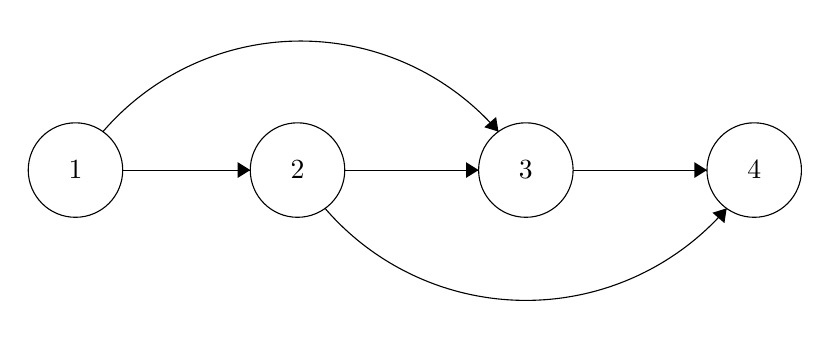
\begin{tikzpicture}[scale=0.2]
\tikzstyle{every node}+=[inner sep=0pt]
\draw [black] (16.1,-27.9) circle (3);
\draw (16.1,-27.9) node {$1$};
\draw [black] (30.2,-27.9) circle (3);
\draw (30.2,-27.9) node {$2$};
\draw [black] (44.7,-27.9) circle (3);
\draw (44.7,-27.9) node {$3$};
\draw [black] (59.2,-27.9) circle (3);
\draw (59.2,-27.9) node {$4$};
\draw [black] (19.1,-27.9) -- (27.2,-27.9);
\fill [black] (27.2,-27.9) -- (26.4,-27.4) -- (26.4,-28.4);
\draw [black] (33.2,-27.9) -- (41.7,-27.9);
\fill [black] (41.7,-27.9) -- (40.9,-27.4) -- (40.9,-28.4);
\draw [black] (47.7,-27.9) -- (56.2,-27.9);
\fill [black] (56.2,-27.9) -- (55.4,-27.4) -- (55.4,-28.4);
\draw [black] (17.843,-25.463) arc (139.24738:40.75262:16.577);
\fill [black] (42.96,-25.46) -- (42.81,-24.53) -- (42.06,-25.18);
\draw [black] (57.453,-30.334) arc (-40.77401:-139.22599:16.84);
\fill [black] (57.45,-30.33) -- (56.55,-30.61) -- (57.31,-31.27);
\end{tikzpicture}
\end{center}

\noindent However, one natural limitation of this model is the following theorem:

\begin{theorem}
A graph $G$ has a topological ordering if and only if it is a DAG (directed acyclic graph).
\end{theorem}
\begin{proof}
See Section 3.6 of Algorithms Design by Kleinberg and Tardos.
\end{proof}

\noindent To solve this issue, we think of two algorithms. One is to reduce the originial graph into a DAG: keep removing the most "unimportant" edges untils the graph is acyclic. By most "unimportant" we then have to find a way to measure the importance of an edge. In this model, the weight (or importance) an edge by the net-loss it is associated with:

$$w(e_{i, j}) = \mbox{number of times j beats i} - \mbox{number of times j beats i}$$

\noindent The algorithm then works as following:

\vspace{5mm}

%\begin{algorithm}[H]
%\begin{algorithmic}
%\While{$G$ is not DAG}
%\State{$e_{min} = \argmin_{e \in E} w(e)$}
%\State{Remove $e_min$ from $G$}
%\EndWhile
%\end{algorithmic}
%\end{algorithm}

\vspace{5mm}

\noindent However, this algorithm has apparent flaws: suppose even though coach A and coach B only encounter each other once, however it is in the SuperBowl, while the matchup between coach A and coach C is quite often but only in friendly games or early-season games and therefore the result is less important and less indicative of their comparative abilities. Therefore using the net-loss as the only measurement of the importance of an edge can possibly remove the important edge and keep the unimportant ones. We can of course tweak the edge-weight by introducing the importance of a game, the time in both coaches' career when the match happens, etc., but simply adding heuristics seem not like the best approach to the problem.
\\

\noindent The second algorithm requires a certain "leap of faith" by introducing randomness into our model:

\subsubsection{Markov Chain (Voting Model)}

To solve the problem of Topogical Ordering, instead of trying to create a DAG to fit the algorithm, we decide adjust the mechanism behind ranking using Topological Ordering.
\\

\noindent Imagine instead of having us, the spectators doing the voting and the ordering, each coach will have a $\bf{vote}$ of a certain $\bf{size}$, which she can divide up into pieces. She can then give the chunks of the vote to different coaches which she think is definitely better coach than she is. We assume the coaches to be rational: she doesn't take into account the opinions of amateurs and public media, and only give out votes to the one she truly believe is better than her (one possible way is only give out vote to the coaches who has beaten her). Then we will rank the coaches based on how many votes each coach eventually get. However since the coaches form a graph and there even might be cycles in the game, so at each timestep a coach can be both receiving and giving. What we are interested in is the distribution of the votes at some large time.
\\

\noindent Consider the following example. There are four coaches: 1, 2, 3, 4. Coach 1 has been beaten by 1 and 4, coach 2 has been beaten by 3 and 4, coach 3 has been beaten by 4 and 1, coach 4 has never been beaten.

\begin{center}
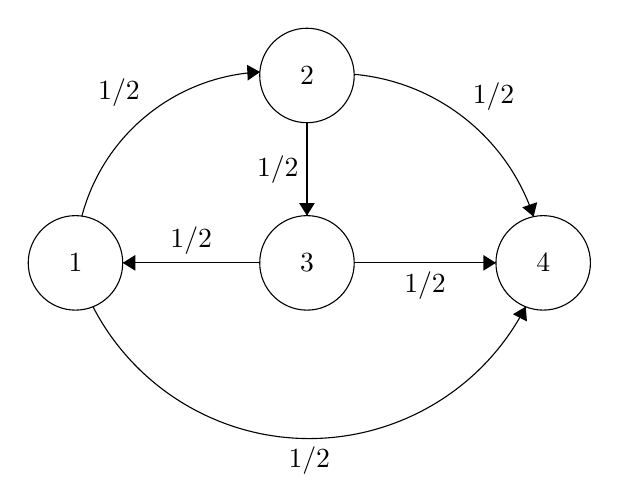
\begin{tikzpicture}[scale=0.2]
\tikzstyle{every node}+=[inner sep=0pt]
\draw [black] (37.8,-30.2) circle (3);
\draw (37.8,-30.2) node {$3$};
\draw [black] (23.1,-30.2) circle (3);
\draw (23.1,-30.2) node {$1$};
\draw [black] (37.8,-18.3) circle (3);
\draw (37.8,-18.3) node {$2$};
\draw [black] (52.8,-30.2) circle (3);
\draw (52.8,-30.2) node {$4$};
\draw [black] (51.691,-32.982) arc (-27.29025:-152.70975:15.462);
\fill [black] (51.69,-32.98) -- (50.88,-33.46) -- (51.77,-33.92);
\draw (37.95,-41.86) node [below] {$1/2$};
\draw [black] (23.506,-27.235) arc (165.22297:92.75902:12.309);
\fill [black] (34.82,-18.08) -- (33.99,-17.62) -- (34.04,-18.62);
\draw (25.86,-20.31) node [above] {$1/2$};
\draw [black] (40.793,-18.226) arc (84.9222:18.22552:13.234);
\fill [black] (52.19,-27.27) -- (52.42,-26.35) -- (51.47,-26.67);
\draw (49.65,-20.55) node [above] {$1/2$};
\draw [black] (34.8,-30.2) -- (26.1,-30.2);
\fill [black] (26.1,-30.2) -- (26.9,-30.7) -- (26.9,-29.7);
\draw (30.45,-29.7) node [above] {$1/2$};
\draw [black] (40.8,-30.2) -- (49.8,-30.2);
\fill [black] (49.8,-30.2) -- (49,-29.7) -- (49,-30.7);
\draw (45.3,-30.7) node [below] {$1/2$};
\draw [black] (37.8,-21.3) -- (37.8,-27.2);
\fill [black] (37.8,-27.2) -- (38.3,-26.4) -- (37.3,-26.4);
\draw (37.3,-24.25) node [left] {$1/2$};
\end{tikzpicture}
\end{center}

\noindent The Markov Chain above shows how the vote will be given out at each timestep: coach 1 will give out half of her vote to coach 2 and the other half to 3, coach 2 will give out half of her vote to coach 3 and the other half to coach 4, coach 3 will give out half of her vote to coach 1 and the other half to coach 4. Coach 4, since she never lost to anyone, will simply keep her vote to herself. We can therefore see this can be modeled as a Markov Chain, and the distribution of votes at some large time is the stationary probability distribution of this Markov Chain:

$$ \pi = \lim_{n \rightarrow \infty} \phi_{0} P^n \mbox{ for some initial distribution } \phi_{0}$$

\noindent where $\bf{P}$ is the probability transition matrix, with $\bf{P}_{i,j}$ equal to the proporption of her chunk coach i will give to j (can also be interpreted as the probability of going from i to j in the Markov Chain):

\[
\bf{P} = 
\begin{bmatrix}
0 & 0.5 & 0.5 & 0 \\
0 & 0 & 0.5 & 0.5 \\
0.5 & 0 & 0.5 & 0 \\
0 & 0 & 0 & 1
\end{bmatrix}
\]

\noindent We know that if the Markov Chain is irreducible and aperiodic, then such a stationary distribution exists, and is unique, and it is the left eigenvector of $\bf{P}$ for the eigenvalue 1.


\subsubsection*{Irreducible \& Aperiodic}

\noindent Apparently, the example we show doesn't satisfy the property. To make sure the matrix we encounter will be irreducible and aperiodic, we use a similar technique as the PageRank algorithm used by Google:

\begin{enumerate}
\item For dead-ends (coach 4 in the example), in each step she will split her vote into equal pieces and give one piece to every coach, (go to a random state in the Markov Chain)
\item For non-deadends (coach 1, 2, 3 in the example), in each step with he will first split her vote into two, with proportion $\alpha$ and $1 - \alpha$. With the $\alpha$ proportion she did what she did before, spliting it and give the pieces to coaches who have beaten her, the remaining $1 - \alpha$ she will split into equal pieces and give one piece to every coach.
\end{enumerate}

\noindent Therefore, after adjusting for deadends in ${\bf P}$, the new probability transition matrix can be represented as:

$${\bf D} = \alpha {\bf P} + (1 - \alpha) {\bf U}$$

\noindent where $\bf{U}$ with all entries equal to $\frac{1}{n}$, $n$ being the total number of coaches (or number of states in the Markov Chain).
\\

\noindent With the new probability transition matrix, since all entries in $\bf{D}$ are positive, we know by Perron-Frobenius theorem that $\bf{D}$ is both irreducible and aperiodic, and that the stationary distribution $\pi$ exists and is unique. With $\pi$ we can find the coaches with the top $5$ probability and they will be the best coaches "of all time" since they get the most proportion of votes from all coaches in the long-run.

\subsubsection*{Formal Representation}

$$G(V, E) \mbox{ represents the graph of coaches}$$
$$V = \{v_1, v_2 ... v_n\} \mbox{ where } v_i \mbox{ is coach i }$$
$$(v_i, v_j) \in E : \mbox{ coach j beats coach i more often than coach i beats coach j }$$



\[
    {\bf P} (i, j)= 
\begin{cases}
    \frac{ I\{(v_i, v_j) \in E\}}{d(v_i)},& \text{if } d(v_i) \geq 1\\
    \frac{1}{n},              & \text{otherwise}
\end{cases}
\]

$${\bf D} (i, j) = \alpha {\bf P} (i, j)  + (1-\alpha)\frac{1}{n}$$


\subsubsection*{Efficient Implementation}


Since the matrix ${\bf D}$ is huge and all entries are non zero, calculating its eigenvalues and eigenvectors directly can be very inefficient computationally. However ${\bf P}$ is a sparse matrix and most of its entries are zero. To make sure we will be able to produce the eigenvector that represents the stationary distribution efficiently, we use Power Method:

\vspace{5mm}

%\begin{algorithm}[H]
%\begin{algorithmic}
%$v = (1/n, ... ,1/n)$\;
%\While{$\| \alpha v {\bf P} + (1 - \alpha)(1, ... ,1) - v\|_2 < e^{-8}$}
%\State{$v = \alpha v {\bf P} + (1 - \alpha)(1, ... ,1)$}
%\EndWhile
%\Return{$v$}
%\end{algorithmic}
%\end{algorithm}

\vspace{5mm}

\noindent Since $v {\bf P}$ can be calculated using sparse matrix ${\bf P}$, this algorithm is much more computationally efficient than simply calculating the eigenvectors of ${\bf D}$. As $\alpha$ increases, the time it takes for $v$ to converge is shorter, but the difference in the ranking might be less significant, therefore this is a tradeoff and we pick $\alpha = 0.95$.

\subsubsection*{Edge Weights}

\noindent In the model we introduced above, in situation where $d(v_i) \geq 1$ (which is something we assume in the rest of this section), ${\bf P}(i, j) = \frac{ I\{(v_i, v_j) \in E\}}{d(v_i)}$, where $I\{(v_i, v_j) \in E\}$ is simply an indicator variable indicating whether i has a net-loss against j. However there are a lot more information we can capture, if we think more about the vote coach i will give:

\begin{enumerate}
\item Game's importance: The more important the game is, the more effort both coaches will put in, and therefore the game result will be more convincing and informative, and more likely coach $i$ will be to give the vote to coach $j$, had coach $i$ lost.
\item Time in Career: If it is early in the career of coach $i$ when he lost to coach $j$, she is going to put less weight than the game she lost later in her career, since it is typical for a coach to learn from failure early and become a better coach later. Therefore coach $i$ will be more convinced to give vote to someone she lost to later in her career.
\item Game Score: A game lost very close is definitely less convincing than a game entirely dominated by opponent. Therefore the more score coach $i$ lost, the more convinced she will be to give your vote to your opponent.
\end{enumerate}

\noindent There are definitely more information that can be informative, however due to the difficulty of data-mining and significance comparison, we come up with the following updated formula to calculate the weight for edge weight:
\\

\noindent Let $T$ be the set of all games
\\
$f: T \rightarrow \mathbb{R}$ map a game to the score difference of the game (positive winning score, 0 if draw)
\\
$h: T \rightarrow \mathbb{I}$ returns the importance multiplier of a game, it is sport specific since different sport have different game structure.
\\
$\beta: $ the score difference adjustment, it is specific to a type of sport. For example, in basketball $\beta$ is set to be smaller than in soccer since the score difference in basketball is much larger. 

$$ T_{i,j} = \{t \in T : \mbox{ coach i lost to coach j in } t\} $$
$$w(v_i, v_j) =  \max(0, \sum_{t \in T_{i, j}} h(t) \log(1 + \beta f(t)) - \sum_{t \in T_{j, i}} h(t) \log(1 + \beta f(t))) $$
$$(v_i, v_j) \in E \mbox{ if } w(v_i, v_j) > 0$$

\[
    {\bf P}(i, j)= 
\begin{cases}
    \dfrac{w(v_i, v_j)}{\sum_{w(v_i, v_k) > 0} w(v_i, v_k)},      & \text{if } d(v_i) \geq 1\\
    \frac{1}{n},              & \text{otherwise}
\end{cases}
\]
\\

\noindent The intuition for this formula is really straightforward: for example, if a coach lost 30 points in Super Bowl, it definitely is going matter much more than a loss of 4 points in an early-season game. The weight for an edge is just a combination of the two factors: the importance of the game, and the score difference of the loss.

\subsubsection*{Parameter Estimation}
\noindent $f:$ we approximate $f$ it to be $\frac{1}{\mbox{maximum number of such game a team can play per season}}$. The reason for this approximation is clear, the less frequent a type of sub-game is, the more it is valued. In NCAA, a team 30 season games, 5 tournament games, and 1 championship game, therefore $h(\mbox{season}) = \frac{1}{30}$, $h(\mbox{tournament}) = \frac{1}{5}$, $h(\mbox{championship}) = 1$. Similarly, in College Football, $h(\mbox{season}) = \frac{1}{12}$, $h(\mbox{playoff}) = \frac{1}{2}$, $h(\mbox{championship}) = 1$
\\

\noindent $\beta:$ it is set to be the inverse of the medium score difference of a sport in the data. From the data, we calculated the median and set $\beta_{basketball} = \frac{1}{9}$, $\beta_{football} = \frac{1}{10}$. We do not use the mean because there are outliers in the score difference in its distribution, as we can see in the following graph:
\\

\begin{figure}[H]
      \centering
      \begin{subfigure}{0.48\textwidth}
      \caption{Distribution of Basketball Score Difference}
      \centering
      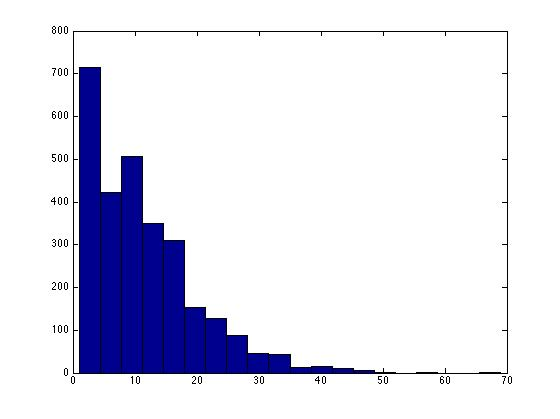
\includegraphics[width=1.1\textwidth]{graphs/basketball_diff_dist.jpg}
      \end{subfigure}\quad
      \begin{subfigure}{0.48\textwidth}
      \caption{Distribution of Football Score Difference}
      \centering
      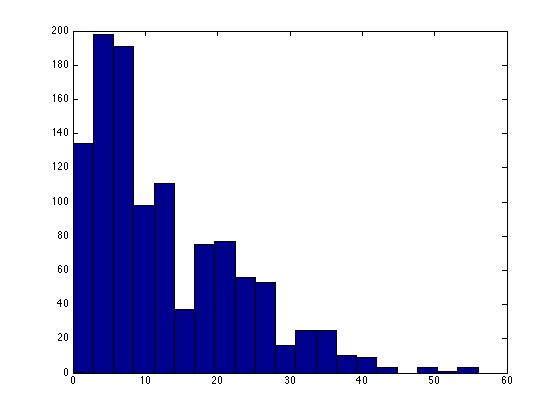
\includegraphics[width=1.1\textwidth]{graphs/football_diff_dist.jpg}
      \end{subfigure}
 \end{figure}

\noindent 
\\

\noindent There are a lot more possible variation with edge weights in the graphical model. However as more detailed information is added into the model, the less significant difference it is going to make, especially among the top results returned, where the differences between coaches are already quite large. Therefore due to time constraint the above model and method of parameter estimation is the final version we decided to use for our graphical approach. As we can see in later sections, the results are promising.

\subsection{Machine Learning Model}

However, for some type of sports, there are not usually data available for every game this coach played against other coaches. We therefore need to come up of ways to deal with small-data.

\section{Results \& Validation}

In this section we are just giving the results of the top-5 coaches for 3 sports. The 3 sports we choose are Male College Basketball, Male College Football, and Male College Baseball. We will start with the result using the Non-connected Model.

\subsection{Result of Non-connected Model}

\subsubsection*{Male College Basketball}

\begin{center}
\begin{tabular}{ | c | c | c| c |}
\hline
Coach Name       & Wins  & Loss & Wilson Score \\\hline
Adolph Rupp      & 876   & 190  & 0.8210 \\\hline
John Wooden      & 664   & 162  & 0.8030 \\\hline
Roy Williams     & 715   & 187  & 0.7918 \\\hline
Jerry Tarkania   & 761   & 202  & 0.7894 \\\hline
Dean Smith       & 879   & 254  & 0.7750 \\
\hline
\end{tabular}
\end{center}

\subsubsection*{Male College Football}

\begin{center}
\begin{tabular}{ | c | c | c| c |}
\hline
Coach Name       & Wins  & Loss & Wilson Score \\\hline
Tom Osborne      & 255   & 49   & 0.8374 \\\hline
Bear Bryant      & 323   & 85   & 0.7904 \\\hline
Bo Schembechler  & 234   & 65   & 0.7811 \\\hline
Wallace Wade     & 171   & 49   & 0.7755 \\\hline
Woody Hayes      & 205   & 61   & 0.7691 \\
\hline
\end{tabular}
\end{center}

\subsubsection*{Male College Baseball}

\begin{center}
\begin{tabular}{ | c | c | c| c | }
\hline
Coach Name       & Wins   & Loss & Wilson Score \\\hline
Ed Cheff         & 1705   & 430  & 0.7980 \\\hline
Mike Martin      & 1771   & 611  & 0.7429 \\\hline
Gene Stephenson  & 1837   & 675  & 0.7307 \\\hline
Augie Garrido    & 1874   & 871  & 0.6821 \\\hline
Gordie Gillespie & 1893   & 952  & 0.6648 \\
\hline
\end{tabular}
\end{center}

\noindent Since this model only takes into account a coach's career win and loss, the result will differ a lot from the graphical model, which capture more information:

\subsection{Result of Graphical Model (Voting Model)}

Using the Markov Chain model with the edge weight function that takes game's importance, and score difference into account, we computed the following result and showed the top five coaches for Male College Football and Male College Basketball (due to time-constraint, we were not able to find game data for College Male Baseball to form a graph):

\subsubsection*{Male College Football}

\noindent The graph $G(V, E)$ for Male College Football have 529 nodes, 1032 edges, and 27 weakly connected component. The fact that there is no one single connected component is possibly due to the small size of our dataset. The top five coaches are:

\begin{center}
\begin{tabular}{ | c | c | }
\hline
Coach Name   & Vote \% \\\hline
Joe Paterno  & 0.02421 \\\hline
Mack Brown   & 0.01728 \\\hline
Bear Bryant  & 0.01663 \\\hline
Lloyd Carr   & 0.01491 \\\hline
Pete Carroll & 0.01338 \\
\hline
\end{tabular}
\end{center}

\subsubsection*{Male College Basketball}

\noindent The graph $G(V, E)$ for Male College Basketball have 763 nodes, 2582 edges, and 1 weakly connected component. The fact that $G$ is weakly connected is really useful in that it allow us to compare every two coaches in the graph, even though they are playing in different time horizon. The top five coaches are:

\begin{center}
\begin{tabular}{ | c | c | }
\hline
Coach Name  & Vote \% \\\hline
Mike Krzyzewski & 0.03272 \\\hline
Dean Smith  & 0.02544 \\\hline
Roy Williams & 0.02329 \\\hline
John Wooden  & 0.02170 \\\hline
Rick Pitino  & 0.02066 \\
\hline
\end{tabular}
\end{center}

\noindent If we plot the Vote \% of all the coaches from high to low, we can get the following histogram:

\begin{figure}[H]
      \centering
      \begin{subfigure}{1\textwidth}
      \caption{Male College Football Vote \%}
      \centering
      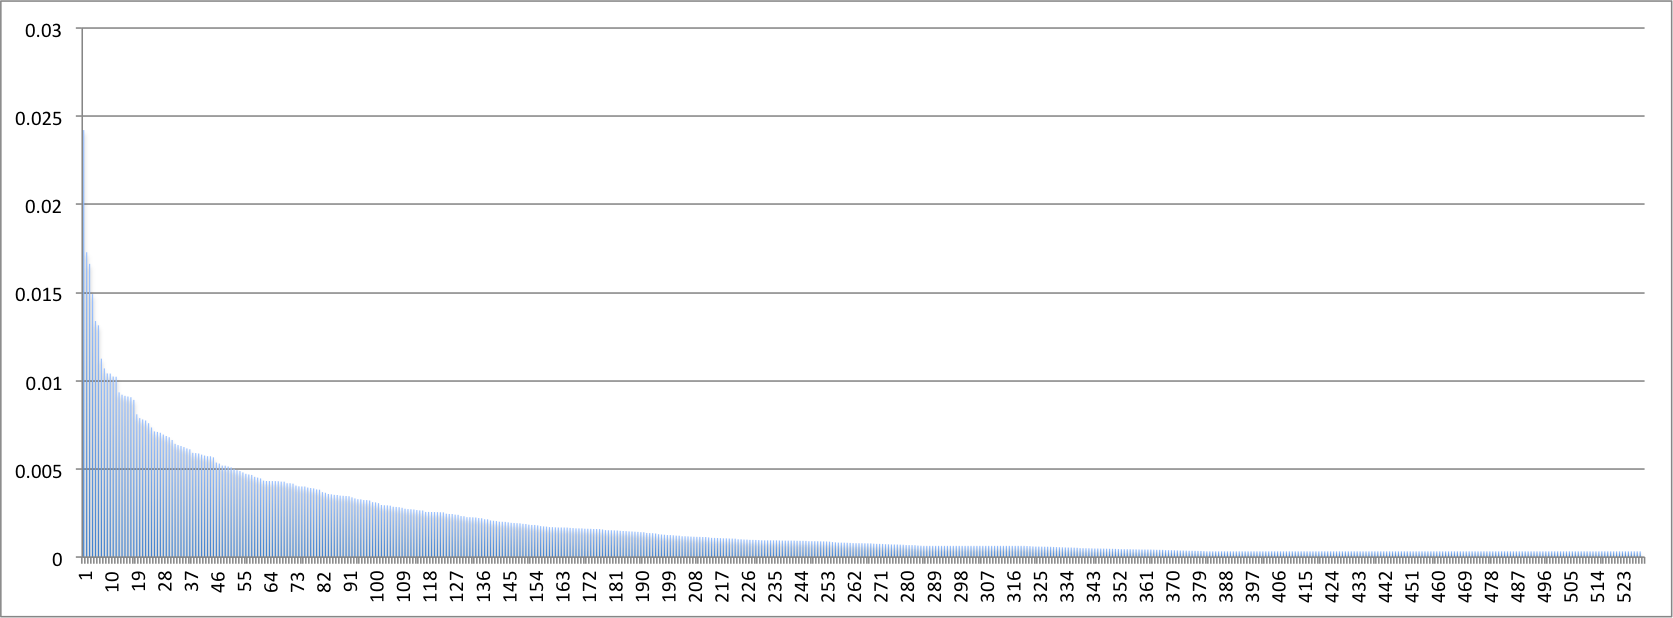
\includegraphics[width=1.1\textwidth]{graphs/football_score_dist.png}
      \end{subfigure}
      \begin{subfigure}{1\textwidth}
      \caption{Male College Basketball Vote \%}
      \centering
      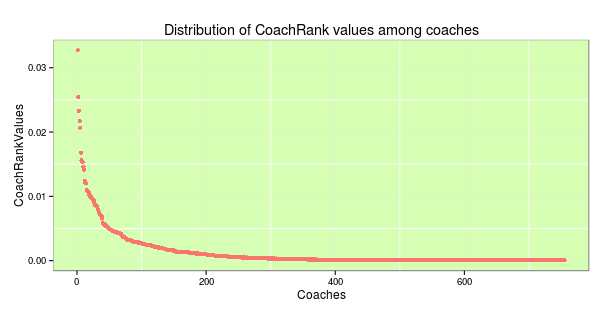
\includegraphics[width=1.1\textwidth]{graphs/basketball_score_dist.png}
      \end{subfigure}
 \end{figure}

\noindent Comparing the two graphs, we can see some clear similarities and differences.

\begin{enumerate}
\item The curve drops off very quickly, which means there are large differences between coaches with the top votes.
\item A small proportion of coaches hold the majority of the votes. In Male College Basketball, $5.6\%$ of the coaches hold $50\%$ of the votes. In Male College Football, $12.4\%$ of the coaches hold $50\%$ of the votes.
\item The graph for football have fatter tails than the graph for basketball, indicating that the vote are more spread out. This is a valid result since there are much more uncertainty in football than in basketball.
\end{enumerate}

\subsubsection*{Assessment}

\noindent Due to the subjective nature of this problem, assessment of the result can be trickly. By comparing both of our results with public polls and professional sports media, and looking at the achievements of coaches returned, we conclude that the result is consistent with public opinions.

\subsubsection*{Robustness}

\noindent Varying parameters $\alpha$ from 0.75 to 0.95, and scaling $\beta$ upwards and downwards by $10\%$, the top 5 coaches returned doesn't have much difference, just with minor rank movement among the top 10 coaches. This is in part due to the quick drop-off rate of the curve above, and the large score differences between top coaches. Therefore, we conclude that the result of the graphical model is valid and it is robust to change in parameters.

\section{Strengths and Weaknesses}

\subsection{Strengths}
\begin{itemize}
\item The graphical model allow us to be more objective in our ranking algorithm since we can understand it as the coaches voting among themselves based on their game history, instead of arbitrary tweaking of heuristics.

\item We take into account not only the career data of a coach, but also the game result, game score, and the game importance of the games they play against each other.

\item We have efficient implementation using power method to calculate the stationary distribution of the Markov Chain, and the results show clear differentiation between coaches, especially high-ranking ones.
\end{itemize}

\subsection{Weaknesses}
\begin{itemize}
\item Due to the limited amount of data we could collect, we could not consider coaches not in our dataset. For example, John Gagliardi, the coach with the most wins in college Football history, was not in our data set because he competed in the NAIA and NCAA Division III leagues. 

\item Our graphical models used only postseason games as input. We justify this heuristically by saying that only skilled coaches will be play in the postseason. However, this produces somewhat sparse graphs, especially compared to those we could have generated if we were able to collect data on every game.

\item Our data for Baseball does not include any data concerning connections between coaches, therefore we could not use our graph model to choose the best baseball coach. Furthermore, we were unable to collect championship-specific data for Baseball coaches.

\item Assessment is also difficult since ranking is in itself subjective. Our methods of assessment are limited to public polls online, professional sport media, coaches' achievements, and cross-validation between our different models.

\end{itemize}

\section{Conclusions}
Todo

\section{Future work}
\begin{itemize}
\item Obtain more game data and coach career information, and more information about the coaches to train a better model.

\item Come up with an objective mechanism to assess the result of our ranking, such as incorporating more public sources.
\end{itemize}

\pagebreak

\section{Bibliography}
\begin{thebibliography}{9}

\bibitem{Pagerank} Pagerank Algorithm,
\verb|http://ilpubs.stanford.edu:8090/422/1/1999-66.pdf|
\bibitem{Re} $\text{A stochastic optimization model for real-time ambulance redeployment}$,
\\\verb|http://www.sciencedirect.com/science/article/pii/S0305054813000385|
\bibitem{Ithaca} Ithaca Demographics,
\verb|http://www.ci.ithaca.ny.us/maps/index.cfm|
\bibitem{Cornell} Cornell Demographics,
\verb|http://www.cornell.edu/about/facts/stats.cfm|
\bibitem{IC} Ithaca College,
\verb|http://www.ithaca.edu/admission/facts/|


\end{thebibliography}

\end{document}